\section{Literature review Methodology} %zs
This chapter aims to systematically review and analyze the current research status of the field of \textbf{AI-driven DbA}. To ensure the comprehensiveness and rigor of the literature collection process, this study followed the PRISMA guidelines\cite{page2021prisma} for systematic review and conducted a multi-stage iterative evaluation and inclusion process. As illustrate in Fig.\ref{fig:prisma-selection}

\subsection{Data Collection}
\textbf{Identification Stage}:
In the identification stage, this study initially obtained several pieces of literature in applications and technologies of design by analogy (N = 990), AI-driven analogy (N = 104), theory and taxonomy of creative processes (N = 24) through a combination of manual and programmatic retrieval in fields such as human-computer interaction, computer science, design studies, cognitive science, mechanical design and bio-design. After initially identifying a set of literatures, 17 core seed literatures with high citation rates in their respective retrieval fields and high alignment with the direction of this study were identified from the above initial literatures. Subsequently, we conducted forward( N = 30)and backward( N = 30) snowballing on each of themobtaining a total of 658 literature pieces in this process after duplicate removing. In total, 1,615 literatures were collected. The retrieval keywords or phrases used in the corpus construction included ``\textit{Design-by-analogy}'', ``\textit{Analogy Reasoning}'', ``\textit{Analogical Design}'', ``\textit{Case-based Reasoning}'', ``\textit{Analogy Making}''. After deduplication, 1,378 pieces remained. 
\subsection{PRISMA Selection}
\textbf{Screening Stage}:
In the Screening stage, this study ensured the precision of the corpus through multiple filtering processes. First, we used a programmatic approach to quickly identify and eliminate literature that was clearly unrelated to the topic based on titles and abstracts. Subsequently, two researchers independently read and manually screened ambiguous literature. In this stage, we eliminated \textbf{EC1}: literature pieces with duplicate titles ($N = 237$), \textbf{EC2}: those without peer review ($N = 23$), and \textbf{EC3}: irrelevant pieces ($N = 545$), leaving 682 articles in the corpus.

\textbf{Eligibility Assessment Stage}:
In the eligibility assessment stage, two researchers applied a series of explicit exclusion criteria to screen and assess the full text content of potential literature, ensuring the quality of the final corpus. Specifically, we removed: \textbf{EC4}: literature where analogy was merely used as a computational intermediate method with the objective of pure algorithmic analogy research (N = 69); \textbf{EC5}: literature that did not directly serve creative work and processes\cite{hsueh2024counts} (N = 156); \textbf{EC6}: literature that used analogy as an ideational method in domain-specific research but did not delve into its connotation (N = 177); \textbf{EC7}: literature that only validated the effectiveness of DbA and other related empirical studies (N = 91); \textbf{EC8}: literature that did not use broad-spectrum artificial intelligence to drive DbA but relied on other computational methods (N = 59). After this stage, 130 articles remained in the corpus.

\textbf{Inclusion Stage}:
To ensure the thematic relevance and classification coverage of our corpus, the corpus covers all relevant categories, including theory, application, and technology, we strive to ensure an even distribution of literature under each major category. Two author independently using thematic analysis\cite{terry2017thematic} and iterative discussions on the previously screened literature and conduct the taxonomy system, further eliminated 20 pieces that did not meet the research criteria or thematic repetition. A total of 106 literature pieces were retained.
Through the above process and iteration between stages, this study ultimately constructed a highly relevant and representative corpus for the field of AI-driven DbA, with a total of 86 literature pieces included for subsequent literature analysis and review.


\begin{figure}
    \centering
    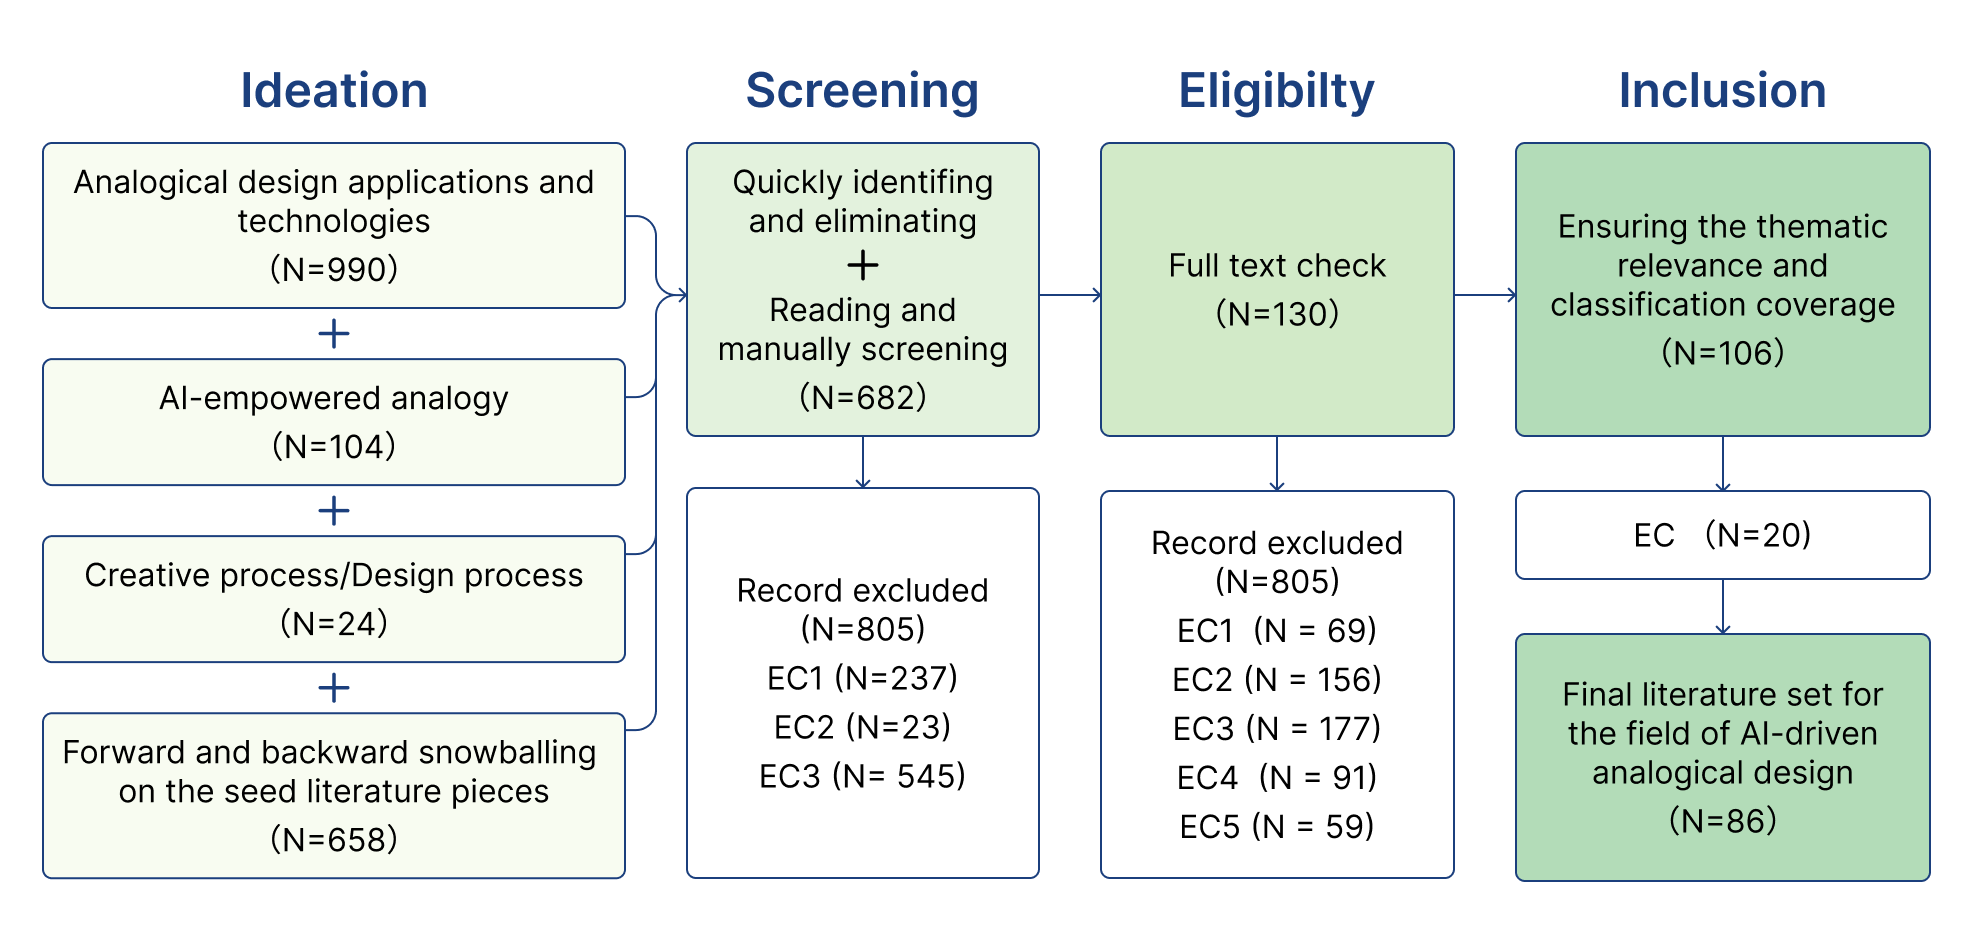
\includegraphics[width=1\linewidth]{Figures/prisma selection.png}
    \caption{This figure presents a literature screening process that adheres to the PRISMA guidelines, detailing the step - by - step filtering of publications across four phases: Collection, Screening, Eligibility, and Inclusion. Explicit exclusion criteria (EC1–EC5, such as duplicate titles, irrelevance, and the absence of peer review) and the changes in the number of publications at each stage are shown. It clarifies how the initial large literature pool (N = 1,816) is gradually refined into a final set of 20 publications that meet the requirements of thematic relevance and methodological rigor.}
    \label{fig:prisma-selection}
\end{figure}



%prisma
%相关关键词可以加一些引用,这是前两段内容,第三节也可以逐步写一下

% %本章节旨在系统性地回顾和分析\textbf{AI驱动的类比设计}领域的现有研究现状。为确保文献收集过程的全面性和严谨性,本研究参考系统评价报告指南PRISMA流程进行多阶段迭代评估及纳入。具体而言,文献筛选过程主要分为识别阶段、筛选阶段、资格评估阶段和最终纳入阶段。

% 识别阶段:
% 在识别阶段,本研究首先通过手动收集和程序化检索相结合的方法,在人机交互、计算机、设计学、认知科学、机械设计、生物设计等领域初步获得了类比设计相关应用及技术文献990篇、人工智能赋能的类比相关文献104篇、创意过程/设计流程相关文献24篇。同时,在初步识别一系列文献后,我们从上述初始文献中,识别出17篇在各自检索领域内引用率较高且与本研究方向高度契合的核心种子文献(如图?所示),随后对这些种子文献进行了程序化的前向和后向滚雪球,各30篇,此过程共获得文献658篇。共计1,615篇,去重后1378篇,检索中使用的核心关键词或词组包括Design-by-analogy、Analogy Reasoning、Analogical Design、Case-based Reasoning、Analogy Making,文献检索的时间范围设定在1983年至2025年。
 
% 筛选阶段:
% 在筛选阶段,本研究通过多重过滤筛选确保文献库的精准性。首先,我们使用程序化方式根据标题和摘要快速识别并剔除与主题明显不相关的文献。随后,2名研究人员对一些模糊文献进行逐一独立阅读和人工筛选。此阶段剔除了标题重复的文献237篇、未经同行评审的文献23篇、无关文献545篇,文献池剩余文章682篇。 

% 资格评估阶段:
% 在资格评估阶段,2名研究人员应用了一系列明确的排除标准对潜在文献进行了逐篇全文内容筛查及评估,从而保障最终文献库的质量。具体而言,我们剔除了移除了:EC1 类比仅作为计算中间环节,用户无法感知到的纯粹算法类比研究(N = 69);EC2 文献不直接服务于创造过程, 参考hsueh et al.提出的创造工作定义\cite{hsueh2024counts}的文章(N = 156);EC3 文献在研究方法中使用类比这一方法但未深入探讨其内涵的文献(N = 177);EC4 文献仅验证类比设计有效性及其他相关实证研究的文章(N=91),EC5 应用文献没有使用广义的人工智能进行类比设计驱动而是用其他方式(N = 59)此阶段文献池剩余文章130篇。 

% 最终纳入阶段:
% 为了确保最终文献库在主题相关性与分类覆盖度上差异分布,文献库需尽可能涵盖所有相关的分类,包括理论、应用和技术,并力求保证每个主要分类下文献分布均匀,共保留文献106篇。在建立分类法后,我们对前期筛选出的文献进行了主题审阅和讨论,并进一步剔除了20个不符合研究标准的文献。   
% 通过上述系统性、多阶段的文献收集和筛选过程,本研究最终构建了一个与AI驱动的类比设计领域高度相关且具有代表性的文献集合,最终纳入了86篇文献用于后续的文献分析和综述。 
\subsection{Corpus Overview}
%本研究通过系统性的多阶段筛选流程,构建了一个包含86篇文献的语料库,这些文献在主题相关性、分类覆盖度和研究质量上具有高度代表性。语料库涵盖了从1983年至2025年的研究成果,反映了AI驱动的类比设计领域在不同时期的发展趋势。文献分布均衡地覆盖了理论研究、应用实践和技术方法等多个主要分类,为深入地分析该领域提供了坚实基础。


%可能有一张barchart图